\documentclass[10pt,a4paper]{article}
\usepackage[latin1]{inputenc}
\usepackage{amsmath}
\usepackage{amsfonts}
\usepackage{amssymb}
\usepackage{graphicx}
\usepackage{dirtytalk}
\def\pip{$\pi^+$}
\def\piz{$\pi^0$}
\def\pim{$\pi^-$}
\def\pippim{$\pi^+\pi^-$}
\begin{document}
	\section{Beam Energy Corrections}
\begin{enumerate}
	\item
	\say{Clarify if the photon-energy corrections derived and reported in the note were obtained after the application of the phi-dependent momentum corrections reported in 3.3.1. This correction should be derived after e-loss and phi-dependent momentum corrections are applied.}\\
	Stated on page 75 of the note procedures:\\
	''To validate the corrections of the entire g12 data set, the missing neutron mass was recalculated for each run, shown in Fig. 72, using several correction schemes, i.e. a scheme of just ''energy-loss`` corrections, a scheme of ''energy-loss`` and momentum corrections (JTG PCor), a scheme of ''energy-loss``, momentum corrections (JTG PCor) and beam corrections (MK BeamCor) and a scheme of ?energy-loss? and beam corrections (MK BeamCor). It can be seen in Fig. 72 that the only scheme that sufficed was the combination of ''energy-loss`` and beam corrections.``\\ However, the plot was modified, making the above statement not understandable. In Figure~\ref{fig:beam_cor_progession} below shows the plot that this text is referring to. \\
	It should be noted that one method of deriving the momentum corrections before the beam corrections did not improve either the neutron mass measurement or the proton mass measurement. This can be seen in Figure~\ref{fig:beam_cor_progession} by the red data points. Therefore the beam corrections were derived after e-loss but before the phi-dependent momentum corrections. It also should be noted that after the beam corrections were derived and after the phi-dependent momentum corrections were derived, the beam correction algorithm was re-ran to investigate any possible systematic, however the ratio of the largest derivation, for a run, was on the order of $10^{-4}$ which had only a 0.3~MeV increase at 1~GeV photon beam energy.
	\begin{figure}[h!]\begin{center}
	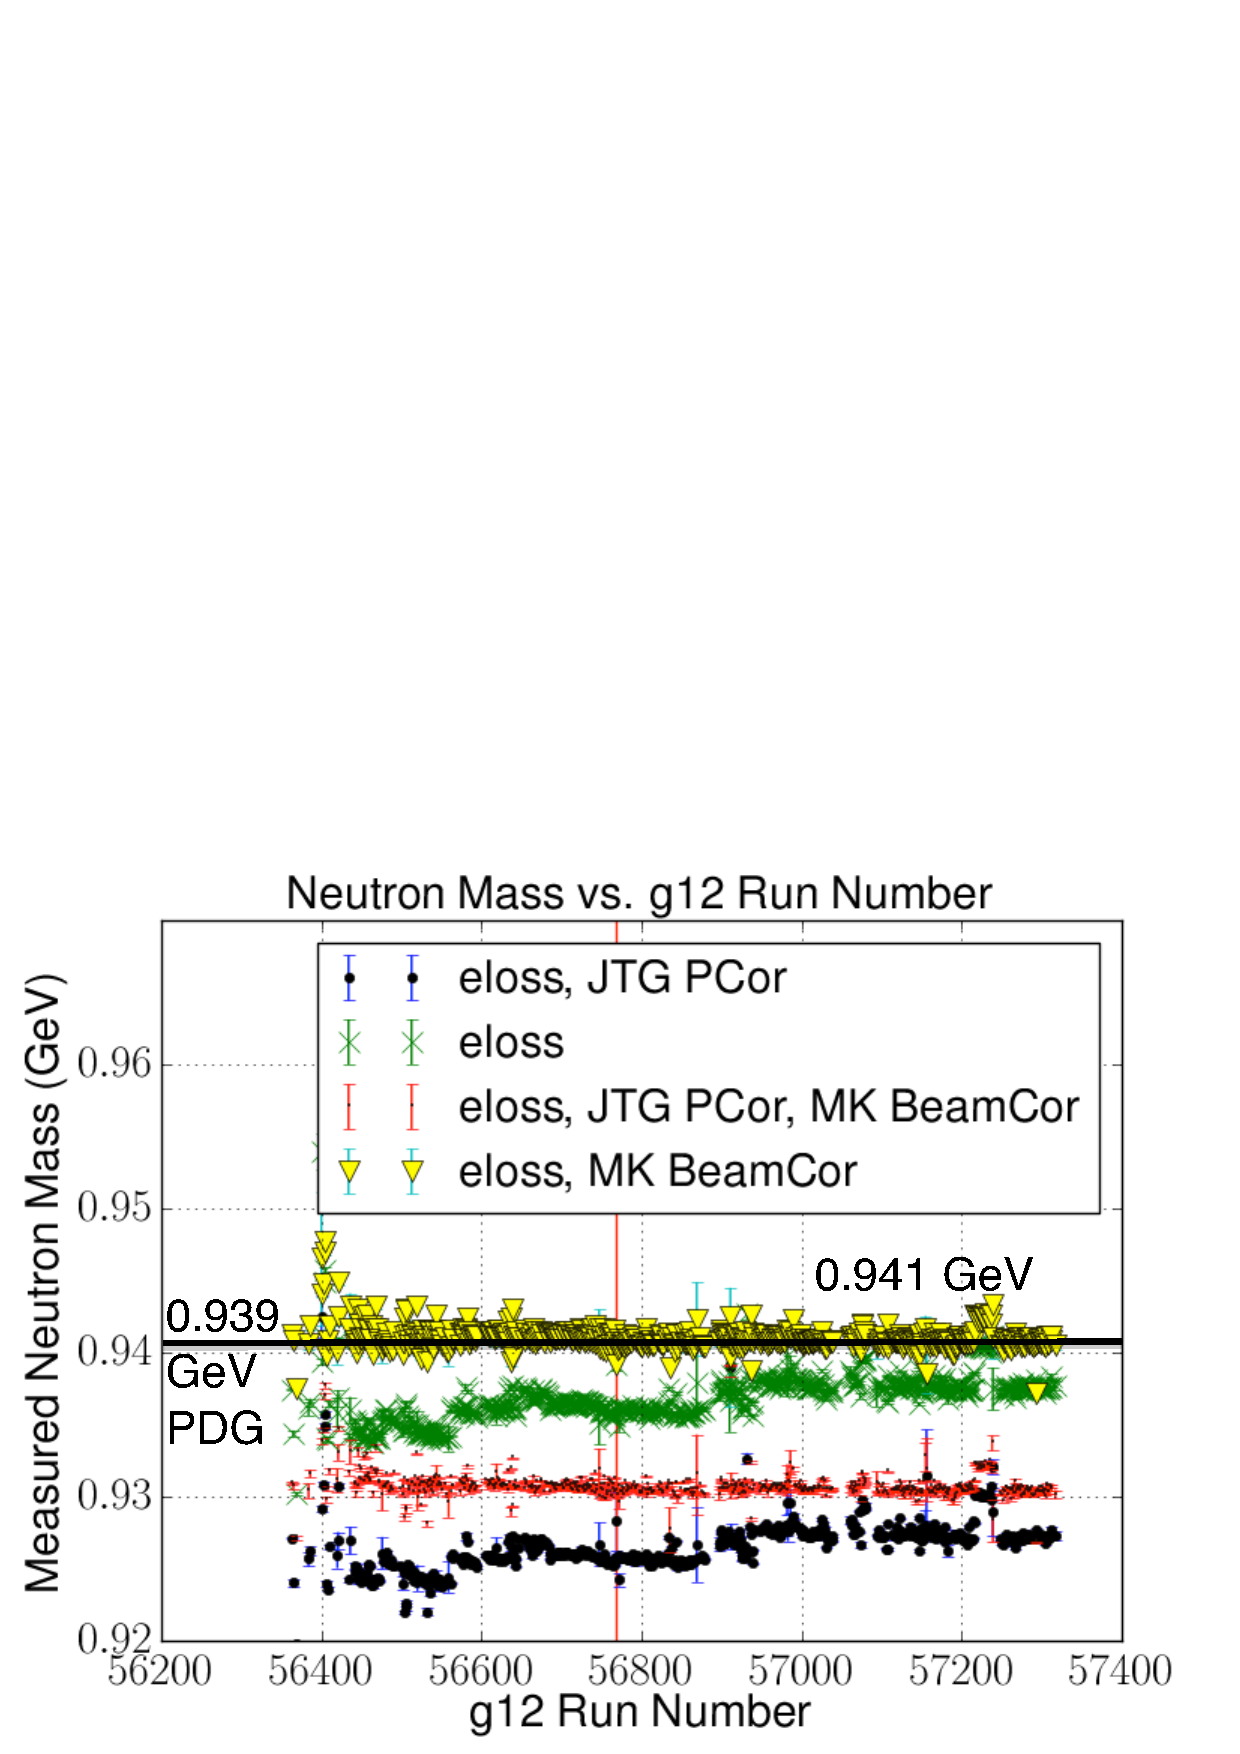
\includegraphics[width=200 pt,height=200 pt]{C3pi_allcorr_neutron_rxr.png}
	 \caption[Plot showing the series of analyses that contributed to the final chain of procedures for the beam correction]{\label{fig:beam_cor_progession}Plot showing the series of analyses that contributed to the final chain of procedures for the beam correction.}
	 \end{center}\end{figure}
	 \item
	 \say{Some of us are concerned that the photon energy correction may absorb any remaining systematic biases in the pion momenta. In such a case, the method by which the photon energy correction is derived ensures that the missing mass peaks are placed right at the nominal mass of the missing particle, but the calculated kinematics at which you report your observables (W, Cm angles) will be incorrectly estimated. We would like to see control distributions that provide evidence that after e-loss and phi-dependent momentum corrections, there are no remaining systematic biases in the particles' momenta:}
	 The observables in which we report (W, C.M. angles) agree well with previous measurements of CLAS and other reputable institutions. However, 
	 \begin{itemize}
	 \item
	 \say{Plot the \pippim invariant mass (Ks) as a function of the \pip and \pim momenta. On each plot show with a solid line the mean of the integrated invariant-mass distribution.}
	 \item
	 \say{Plot the \pippim invariant mass (Ks) as a function of the \pip and \pim theta lab angles. On each plot show with a solid line the mean of the integrated invariant-mass distribution.}
	 \item 
	 \say{Plot the \pippim invariant mass (Ks) as a function of the \pip and \pim common Z vertex. On the plot show with a solid line the mean of the integrated invariant-mass distribution.}
	 \item
	 \say{Plot the \pippim invariant mass (Ks) as a function of run number. On the plot show with a solid line the mean of the integrated invariant-mass distribution.}
	 \end{itemize}
	 
	 
	 
	 as reported in the analysis procedure note, the invariant mass of for 2 run numbers was shown, these 2 run numbers were chosen 
  \end{enumerate}
  
  	\section{Single Particle Efficiency}
  \begin{enumerate}
  	\item
  	\say{The only independent (of analysis) g12 argument at this time that can be acceptable in my view about the validity of the correction would be that after the corrections, the omega cross sections from three-track and two-track events are consistent with each other, but I did not see a comparison of these in MKs thesis}\\
  	In section 4.13.4 of MK thesis, there depicts a comparison of several \piz differential cross-sections from g12 using the dynamic g12 correction compared to the g11 method derived for the g11 experiment. Shown is a good agreement between the 2 methods, however there is slight deviations in the forward $\cos \theta$ direction. We attribute this deviation to the difference in the method of calculating the efficiency, where g12 is dynamic, while the g11 correction was a static ''global`` correction. Furthermore, in the analysis note procedure, the \piz differential cross sections are shown to be in good agreement with previous measurements obtained from CLAS and other world measurements.     \\
  	\item
  	\say{According to MK thesis, the kinematic fit was done after e-loss and beam- energy corrections. Phi-dependent momentum correction was not done. This is not consistent with the analysis chain in the g12 latest note.}
  	It is not explicitly stated, however when kinematic fit is performed, the phi-dependent momentum corrections are performed (Prior to the fit, but in the fit procedure).
  	\item
  	\say{The parameters of the pull distributions of the simulated and the real data are not consistent with each other within their reported uncertainties. (The error matrices for the simu- and real-data fits seem to have been tuned independently. I wonder how the error matrices compare with each other). I suspect that one of the reasons for that discrepancy are residual differences between the resolutions of the simulation and the data. These would not be necessarily caught by comparing integrated distributions, such as invariant and missing masses, but would become prominent as one "zooms" in a particular bin of (p,theta,phi, z).}
  	\item
  	\say{For a better estimate of the magnitude of the issue above, one would need to see differences, such as p_calculated-p_measured for the narrow kinematic bin (theta,phi,z) as a function of momentum (etc), plotted together for simulated and real data (mean values, widths).}
  	\item
  	\say{The counting of detected particles was done by checking if a real particle was detected with kinematics falling within the kinematic bin of interest. On average, that is not a problem, if one derives an overall correction, since bin migration tends to average out. However, that can be very dangerous if the local resolutions in the simulation and the real detector do not match. Different bin migrations will cause a local bias in the efficiency.}
  	\item
  	\say{The uncertainty of the correction has not been estimated (this may take care of my concern in d) as long as the biases are randomly distributed over the (p,theta,phi,z) bins) as far as I could see. The quoted value of 3\% for 3-prong events seems to account for photon multiplicity effects in the correction, but not for inherent effects, such as resolution mismatches simulation-data.}
  	\item
  	\say{In MK's thesis, the detection efficiencies for p, pi+, and pi- are shown both for the simulation and for the data. While, the simulated results nicely show the location of the coils, the real data do not. A relatively high efficiency is
	for the regions of the coils for the data, where we expect zero. One explanation would be that in the determination of the thetacosphi and thetasinphi bins, the bins covering the coil areas contain areas both with zero efficiency and with high efficiency. I would like to see if the efficiency for that bin was reported for the actual average of the events' kinematics in that bin, or the for the middle of the bin (which is unacceptable). I also wonder if the procedure of correction evaluation did check that the actual mean values of the kinematic bins, for which the ratio of efficiencies simu/real was formed, did indeed match, or one trusted the middle of the bins. Again, this may not be an issue for observables reported for wide bins, but brings into question potential errors of the correction (i.e. systematic biases).}
  	\end{enumerate}
  
\end{document}